\documentclass[tikz, border=1cm]{standalone}
\usepackage{ pgfplots, tikz-3dplot}
\usepackage{currfile}
\usetikzlibrary{decorations.text, decorations.markings}
\usetikzlibrary{intersections}
\usetikzlibrary{arrows.meta}  
\usetikzlibrary{shapes, shadows}
\usetikzlibrary{quotes,angles}
\pgfdeclarelayer{bg}    % declare background layer
\pgfsetlayers{bg,main}  % set the order of the layers (main is the standard layer)
\usetikzlibrary{shapes.geometric,calc}
\usepgfplotslibrary{fillbetween}
\pgfplotsset{
	%every tick label/.append style={scale=0.5},
	every axis label/.append style={font=\small},
	compat=newest,
}
\tikzset{every picture/.style={font=\small}}
% -------------------------------------- Електричні кола ------------------------------------------------
\usetikzlibrary{circuits.ee.IEC}
\tikzset{circuit ee IEC,
every info/.style=red,
semithick,
every info/.style={font=\footnotesize},
small circuit symbols,
circuit declare symbol = ampermeter,
circuit declare symbol = voltmeter,
circuit declare symbol = galvanometer,
set ampermeter graphic = {draw,generic circle IEC, minimum size=5mm,info=center:A},%
set voltmeter graphic = {draw,generic circle IEC, minimum size=5mm,info=center:V},
set galvanometer graphic = {draw,generic circle IEC, minimum size=5mm,info=center:G},
}

% -------------------------------------- Grid -------------------------------------------------------
\makeatletter
\def\grd@save@target#1{%
  \def\grd@target{#1}}
\def\grd@save@start#1{%
  \def\grd@start{#1}}
\tikzset{
  grid with coordinates/.style={
    to path={%
      \pgfextra{%
        \edef\grd@@target{(\tikztotarget)}%
        \tikz@scan@one@point\grd@save@target\grd@@target\relax
        \edef\grd@@start{(\tikztostart)}%
        \tikz@scan@one@point\grd@save@start\grd@@start\relax
        \draw[minor help lines] (\tikztostart) grid (\tikztotarget);
        \draw[major help lines] (\tikztostart) grid (\tikztotarget);
        \grd@start
        \pgfmathsetmacro{\grd@xa}{\the\pgf@x/1cm}
        \pgfmathsetmacro{\grd@ya}{\the\pgf@y/1cm}
        \grd@target
        \pgfmathsetmacro{\grd@xb}{\the\pgf@x/1cm}
        \pgfmathsetmacro{\grd@yb}{\the\pgf@y/1cm}
        \pgfmathsetmacro{\grd@xc}{\grd@xa + \pgfkeysvalueof{/tikz/grid with coordinates/major step}}
        \pgfmathsetmacro{\grd@yc}{\grd@ya + \pgfkeysvalueof{/tikz/grid with coordinates/major step}}
        \foreach \x in {\grd@xa,\grd@xc,...,\grd@xb}
        \node[anchor=north] at (\x,\grd@ya) {\pgfmathprintnumber{\x}};
        \foreach \y in {\grd@ya,\grd@yc,...,\grd@yb}
        \node[anchor=east] at (\grd@xa,\y) {\pgfmathprintnumber{\y}};
      }
    }
  },
  minor help lines/.style={
    help lines,
    step=\pgfkeysvalueof{/tikz/grid with coordinates/minor step}
  },
  major help lines/.style={
    help lines,
    line width= 0.5pt,
    step=\pgfkeysvalueof{/tikz/grid with coordinates/major step}
  },
  grid with coordinates/.cd,
  minor step/.initial=.2,
  major step/.initial=1,
  major line width/.initial=2pt,
}
\makeatother
% ------------------------------------ Паттерни -----------------------------------------------------
\usetikzlibrary{patterns}
\tikzstyle{ground}=[fill,pattern=north east lines,draw=none,minimum width=0.3,minimum height=0.6]

\begin{document}
\begin{tikzpicture}[every pin/.style={minimum size = 5pt, pin edge={red, thick}, draw, fill=gray!5, red, circle, font=\scriptsize},
    small dot/.style={fill=black,circle,scale=0.3}]
    \node at (0,0){ 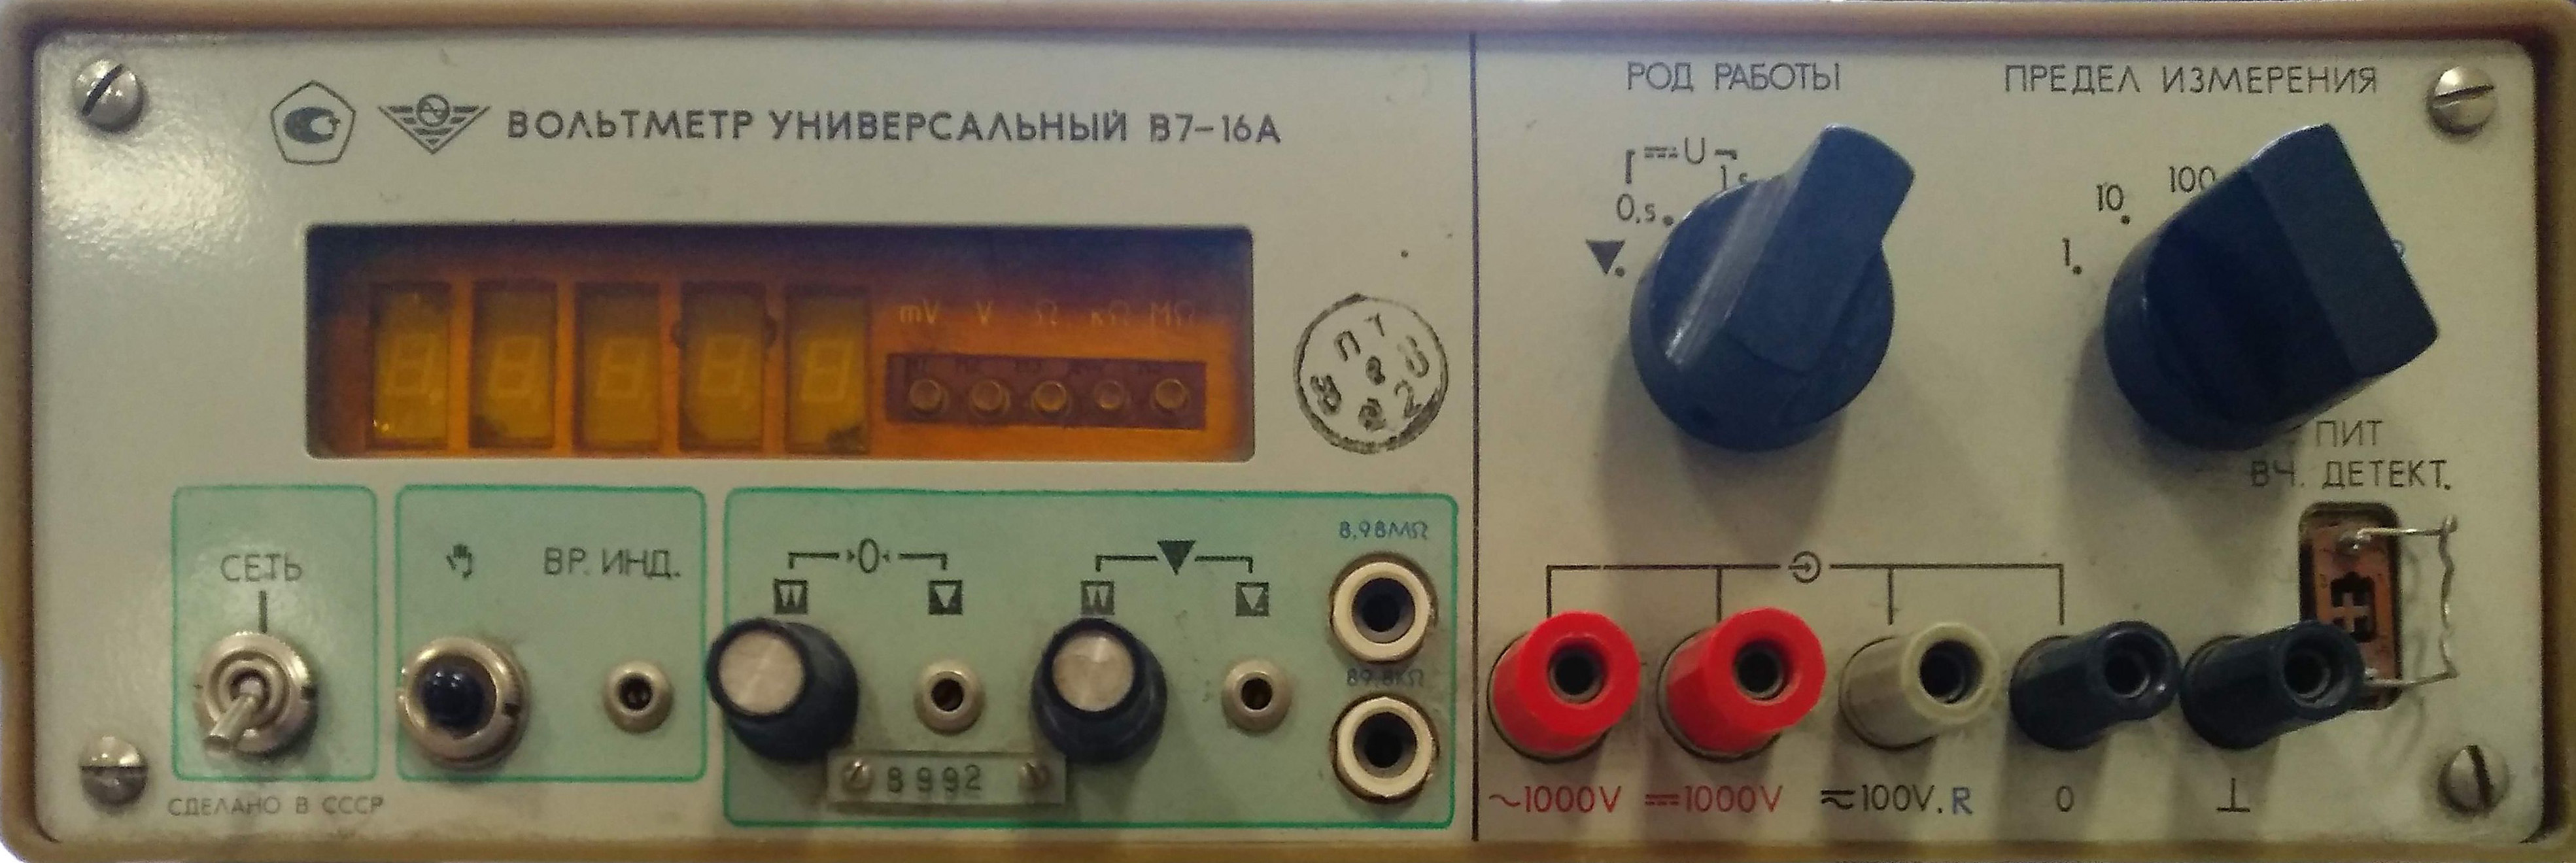
\includegraphics[width=12cm]{V716A}};
    \node[small dot,pin={[pin distance=0.8cm]-90:{\ref{btn:powerV716A}}}] at (-4.9,-1.3) {};
    \node[small dot,pin={[pin distance=1cm]-90:{\ref{btn:O}}}] at (-2.5,-1.1)  {};
    \node[small dot,pin={[pin distance=1cm]-90:{\ref{btn:Tri}}}] at (-0.9,-1.1)  {};
    \node[small dot,pin={[pin distance=1.5cm]90:{\ref{btn:Rod}}}] at (2.4,0.6)  {};
    \node[small dot,pin={[pin distance=1.5cm]90:{\ref{btn:Limit}}}] at (5,0.6)  {};
    \node[small dot,pin={[pin distance=1cm]-90:{\ref{pin:AltCur}}}] at (1.35,-1.15)  {};
    \node[small dot,pin={[pin distance=1cm]-90:{\ref{pin:SteadCur}}}] at (2.25,-1.15)  {};
    \node[small dot,pin={[pin distance=1cm]-90:{\ref{pin:Ohm}}}] at (3.1,-1.15)  {};
    \node[small dot,pin={[pin distance=1cm]-90:{\ref{pin:O}}}] at (3.9,-1.15)  {};
    \node[small dot,pin={[pin distance=1cm]-90:{\ref{pin:ground}}}] at (4.8,-1.15)  {};
%    \node[small dot,pin={[pin distance=1.05 cm]-90:{\ref{btn:regexit}}}] at (3.9,-2.1)  {};
%    \node[small dot,pin={[pin distance=1.2cm]180:{\ref{btn:Vscale}}}] at  (-5,0.7) {};
%    \node[small dot,pin={[pin distance=1.1cm]-90:{\ref{btn:VscaleLim}}}] at  (-4.2,-2) {};
%    \node[small dot,pin={[pin distance=1.1cm]90:{\ref{scale:Vscale}}}] at (-2.8,2) {};
%    \node[small dot,pin={[pin distance=1.2cm]-90:{\ref{btn:ExtR}}}] at (-1.2,-2) {};
%    \node[small dot,pin={[pin distance=1.6cm]-90:{\ref{btn:IntR}}}] at (-2.3,-1.5) {};
    \draw[red] (-6,-2) to [grid with coordinates] (6,2);
\end{tikzpicture}
\end{document}
